% ---------------------------------------------------------------------
% -------------- PREAMBLE ---------------------------------------------
% ---------------------------------------------------------------------

%\documentclass[12pt,a4paper,english,oneside]{article}
\documentclass[preprint,authoryear,12pt]{elsarticle}

\usepackage[utf8]{inputenc}
\usepackage[english]{babel}

\usepackage{calc}
\usepackage{natbib}
\usepackage{url}
%\usepackage{listings}
\usepackage{hyphenat}

\usepackage{supertabular,array}
\usepackage{lipsum}
\usepackage{booktabs}
\usepackage{graphicx}


% Strike through
\usepackage[normalem]{ulem}

% Punctuation for references
\bibpunct{[}{]}{;}{n}{,}{,}

% correct bad hyphenation here
\hyphenation{op-tical net-works semi-conduc-tor}


% Multiple bibliographies
%\usepackage{multibib}
%\newcites{gen}{References}
%\usepackage{bibentry}


% ---------------------------------------------------------------------
% -------------- DOCUMENT ---------------------------------------------
% ---------------------------------------------------------------------

\journal{Information and Software Technology}

\begin{document}

% Extra definitions?
\selectlanguage{english}

\begin{frontmatter}

%% use the tnoteref command within \title for footnotes;
%% use the tnotetext command for the associated footnote;
%% use the fnref command within \author or \address for footnotes;
%% use the fntext command for the associated footnote;
%% use the corref command within \author for corresponding author footnotes;
%% use the cortext command for the associated footnote;
%% use the ead command for the email address,
%% and the form \ead[url] for the home page:
%%
%% \title{Title\tnoteref{label1}}
%% \tnotetext[label1]{}
%% \author{Name\corref{cor1}\fnref{label2}}
%% \ead{email address}
%% \ead[url]{home page}
%% \fntext[label2]{}
%% \cortext[cor1]{}
%% \address{Address\fnref{label3}}
%% \fntext[label3]{}

%% use optional labels to link authors explicitly to addresses:
%% \author[label1,label2]{<author name>}
%% \address[label1]{<address>}
%% \address[label2]{<address>}

\title{Adopting agile in the large: motivations, success factors and challenges}

\author{Kim Dikert}
\ead{kim-karol.dikert@aalto.fi}

\author{Maria Paasivaara}
\ead{maria.paasivaara@aalto.fi}

\author{Casper Lassenius}
\ead{casper.lassenius@aalto.fi}

\address{Aalto University, School of Science, Department of Computer Science and Engineering}


% ---------------------------------------------------------------------
% ------------------------- ABSTRACT ----------------------------------
% ---------------------------------------------------------------------

\begin{abstract}

Agile methods have become an appealing alternative for companies striving to
improve their performance, but the methods are originally designed for small and
individual teams. This poses challenges when introducing agile to large
organizations where development teams can not be autonomous. We reviewed 30
experience reports and case studies describing the process of taking agile
methods into use in large organizations. The primary motive for agile adoption
is the need to improve performance. For a successful transformation the entire
organization must be aligned and all organizational units must participate.
Creating an agile community in the organization will help the change to stick.
Typical problems are misunderstanding of the agile model, and difficulties
coordinating multiple agile teams.

\end{abstract}

\begin{keyword}
%% keywords here, in the form: keyword \sep keyword
%% MSC codes here, in the form: \MSC code \sep code
%% or \MSC[2008] code \sep code (2000 is the default)

agile \sep transformation \sep large scale \sep adopting agile

\end{keyword}

\end{frontmatter}


% ---------------------------------------------------------------------
% --------------------------- TEXT ------------------------------------
% ---------------------------------------------------------------------


\section{Introduction}

--> Introductory paragraph

--> Motivation for research
-- There are no systematic reviews for this
-- A collection of experience reports can be used for creating a theoretical
   base.
--> There is interest in large scale [ref XP13 workshop]

--> Freudenberg, S. and Sharp, H., "The Top 10 Burning Research Questions from
    Practitioners," IEEE Software, pp. 8-9, 2010.

--> Why is large scale software development different from smaller scale?

--> This literature review is intended for researchers as a theroretical
   and proven foundation for the real problems that organizations face in
   transformations.
   This is also intended to be directly usable by practicioners, to serve as a
   base of general advice with strong motivation (although every organization
   has unique needs).


% ---------------------------------------------------------------------
\section{Background}
\label{sec:background}

Lindvall, M., et al., "Agile Software Development in Large Organizations,"
IEEE Computer, vol. 37, pp. 26-34, 2004.


Boehm, B. and Turner, R., Balancing Agility and Discipline: A Guide for the
Perplexed: Addison-Wesley, 2003.
Boehm, B., "Get ready for agile methods, with care," IEEE Computer, vol. 35,
pp. 64 - 69, 2002.
--> Any hints on size?? Maybe size leaning towards discipline?


% ---------------------------------------------------------------------
\section{Research method}
\label{sec:method}

The goal of the research was to aggregate evidence on how large organizations
transform into an agile way of working. The research was conducted as a
systematic litterature review based on empirical studies.

\subsection{Research questions}

The following research questions were set to guide the research process.

\begin{itemize}

\item
RQ1: Why are transformations initiated?

\item
RQ2: How do transformations usually proceed; do transformations exhibit patterns?

\item
RQ3: What are typical successes and challenges in a large scale agile
    transformation process?

\end{itemize}


\subsection{Definition of large scale}
\label{sec:largescale}

A key question in the study was the definition of \emph{large scale}. Large
scale requires additional coordination and makes communication difficult
compared to software development in small teams.

--> Needs to have complexity in software design?? --> What is complexity in software?
    Is ``complexity'' an issue in agile?
    What will bring complexity into software? Not costs or the length of the
    schedule. --> Having many people will bring the complexity in terms of the
    SDM to use.
--> Some people see cost as a definition for large scale, some see code base
    size [Petersen], some see project duration [Bjarnson?]. These are all
    related, but do not relate to any specific problem. You can spend X amount
    of money, but it does not in itself make any difference if the money is
    spent in an agile way.
--> Formal definitions (EU, etc.) look at project costs or company turnover.
    These definitions do not take a standpoint on complexity of the product, so
    they do not matter in the context of SDMs.

--> Ref: the XP conference
--> [Cockburn 2003] Agile is best suitable for teams around 50 people or fewer.
--> Boehm, B. and Turner, R., Balancing Agility and Discipline: A Guide for the
    Perplexed: Addison-Wesley, 2003. --> There might be a 50 person boundary?
    --> See Boehm also for list of 

--> The company must already be with N teams or N people, not growing up to the
    required numbers. Small companies in growth are therefore excluded. 


\subsection{Research process}

The research was conducted as an application of Kitchenham's
\cite{Kitchenham2007} guidelines for systematic literature review. The selection
of primary studies was done as a keyword based database search and manual
filtering of included studies. The filtering process was executed independently
by two researchers (Dikert, Paasivaara). The selected primary studies were coded
for data extraction and analysis. The entire process was audited by a third
external researcher (Lassenius).

We deviated from Kitchenham's guideline on the part of data extraction. Instead
of using data extraction forms we analyzed the primary studies by coding. This
deviation was made in order to minimize how possible preconceptions would affect
the data extraction step, and to use a specialized software tool that allowed us
to record evidence in as much detail as possible.
% --> Possibility to find many different viewpoinits for the research questions
% --> Lots of items, which would have lead to much diversity in data extraction form 

\subsubsection{Inclusion criteria}
\label{sec:inclusioncriteria}

Based on the research questions and intended focus of the research, we defined
three facets to guide inclusion/exclusion decisions: agile software engineering,
focus on transformation, and large scale. The first facet covers primary studies
focusing on software engineering organizations applying or striving to apply
agile methods. The second facet states that included studies must provide
insights relevant to organizational transformation, and specifically to the
research questions. The third facet underlines the particular contribution we
aim to provide with this research, namely the exclusive focus on large
organizations. These three facets were used for inclusion and exclusion in each
study selection step, including search string design, filtering by abstracts,
and full text filtering.

Examples on topics excluded by the first facet are agile manufacturing, and
applying Scrum practices in management boards. In addition, we required that the
transformation was aimed to introduce agile methods into the studied
organization.

The facet of \emph{organizational transformation} was interpreted so that the
primary study presents insights on the process of transformation. Excluded
topics were: discussing a large agile effort but not presenting the how the
organization had evolved [ref?], pilot cases that clearly span one limited
project [Scott 2008?], and case studies that provide minimal information on the
transformation process [ref?].
--> Transformation and ``scaling up'' are very closely related. In some cases
    they can not really be separated. For instance, if transformation begins
    with a pilot and spreads gradually through the organization, it is very
    likely that the process is seen as a ``scaling up'' journey.
    However, in general, we do not include discussions purely on scaling up,
    especially if no organizational change is considered. [Maranzato 2012, Lyon 2008]

The facet of \emph{large scale} was interpreted as presented in section
\ref{sec:largescale}.
--> Case of one agile team in an enterprise: This is unrelated if the single
    team has no effect on the rest of the enterprise. There is no
    ``organizational transformation'' if there is just one team soloing.  

In addition to the criteria listed above we excluded studies that were not
empirical. We excluded textbooks, studies presenting theories, and other studies
that did not include any case organization. We also excluded student experiments
as it is implausible to simulate the dynamics of a large organization in an
experiment.

% -----------------------

% - pitää olla systemaattinen
% - pitää olla toistettava
% ==> Perustuu enimmäkseen siihen että on 2 tutkijaa toistamassa
% 
% Jos koko on epäselvä:
% --> Tutkijat päättävät keskustelun ja kvalitatiivisen harkinnan perusteella
% --> Tähän tarvitaan esimerkit, milloin on otettu mukaan, milloin on karsittu
%     pois

-- snip --
Listing of not included topics. Discussion on these topics are considered not
providing insight to the research questions. Our goal is to address the research
questions, and specifically focus on analyzing the transformation process.
Not included topics:
--> Benefits of agile in general, problems with agile in general
--> Comparing agile and method X
--> Reporting on the current method, without consideration of how the method has
    been evolved (or transformed)
Tämän perusteella pitää siis kertoa itse prosessista: --> Kirjoita auki tämä
kriteeri paremmin.



\subsubsection{Preliminary searches}

Before proceeding with the keyword search a series of preliminary searches were
performed. Initial searches were made using keywords that were as general as
possible, including ``agile transformation'' and ``large scale agile''.
Additionally, a keyword search was done in the selected databases (listed in
table \ref{table:databases}) using the following search string:

\begin{verbatim}
((agil* OR scrum OR xp OR lean) AND
(transform* OR transit* OR change OR migrat*) AND
((large AND (scale OR organization))) OR enterprise)
\end{verbatim}

From these searches we compiled a list of 117 possibly relevant papers that
should be matched by the keyword searches. The keyword search came to include 75
of the preliminarily selected papers. The missed 32 preliminary papers were
separately examined for inclusion, resulting in including 3 additional papers as
primary studies.

\subsubsection{Study selection}

The study selection process inlcuded three steps, each step refining the set of
selected papers. First a database search was used to gather an initial set of
papers. This set was then refined by filtering out abstracts and finally full
text filtering. The study selection process is outlined in Figure
\ref{fig:selectionprocess}.

\begin{figure}[b]
  \begin{center}
    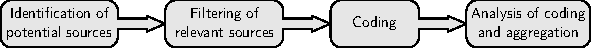
\includegraphics[width=1\textwidth]{graphics/research_process.pdf}
    \caption{Study selection process}
    \label{fig:selectionprocess}
  \end{center}
\end{figure}

A keyword search in online databases was chosen as the means to find potential
primary studies. The databases included in the search are listed in Table
\ref{table:databases}. All databases supported use of complex boolean logic in
searches which allowed us flexibility when constructing the search strings.

\begin{table}
    \begin{tabular}{ p{0.28\textwidth} l l }
        \toprule
        Database         & URL                         & N of matches   \\
        \midrule
        IEEExplore       & http://ieeexplore.ieee.org      & 745 \\ 
        ACM              & http://dl.acm.org               & 168 \\
        Scopus           & http://www.scopus.com/home.url  & 1596 \\
        Web of Knowledge & http://apps.webofknowledge.com  & 786 \\
        \bottomrule
    \end{tabular}
    \caption{Databases included in search, and number of matched articles}
    \label{table:databases}
\end{table}

We constructed a search string based on the facets \emph{agile software
deveolpment} and \emph{organizational transformation}, as presented in section
\ref{sec:inclusioncriteria}. Preliminary searches had showed that picking
keywords with good precision was difficult. Therefore we decided to exclude the
facet \emph{large scale} from the keyword search, with the consequence of
increasing the manual filtering effort in the subsequent steps.
Having a substantial part of the matches in non-relevant areas such as agile
manufacturing, we included only articles including the term ``software'' or
articles published in relevant conferences. Instead of engineering the search
terms any further, which proved to result in excluding some relevant articles,
we chose to rely more on manual filtering. The resulting facets and keywords are
listed in Table \ref{table:searchterms}.

\begin{table}
    \begin{tabular}{ p{0.22\textwidth} p{0.76\textwidth} }
        \toprule
        Facet                  & Keywords   \\
        \midrule
        Agile methods\newline (before \& after) &
            \texttt{agile, scrum, "extreme programming",
            waterfall, "plan-driven", RUP}\\
        Organizational transformation &
            \texttt{transform*, transiti*, migrat*, journey, adopt*, deploy, introduc*,
            "roll-out", rollout}\\
        Only software\newline related atricles &
            \texttt{(software OR (conference="agile, xp, icgse, icse"))
            AND NOT (title+abs="manufacturing" OR conference="agile manufacturing")}
        \\
        \bottomrule
    \end{tabular}
    \caption{Facets and related search terms used}
    \label{table:searchterms}
\end{table}

The database keyword search matched 1874 unique papers. The abstracts of these
papers were categorized independently by both Dikert and Paasivaara into three
categories: include, excude, and uncertain. The result was combined by marking
abstracts both researchers agreed on for inclusion or exclusion respecitvely.
The inclusion of disagreed or uncertain abstracts was resolved through
discussion. At this stage papers were excluded only if both reserachers deemed
it clearly irrelevant, including any uncertain cases for full text filtering. As
a result 170 papers were selected for full text filtering.

% Inter-rater statistics
%
%                     Maria
%            excl   ???   incl    TOT
%      excl  1578    18    15    1611
% Kimi ???     84    17     8     109
%      incl    51    42    62     155
%      TOT   1713    77    85    1875
%
% ???'s =  169
% in/ex = 1706
%
% Pr(Kimi, in) = in / (tot)  =  155 / 1857 = 0.0619
% Pr(Kimi, ex) = ex / (tot)  = 1611 / 1857 = 0.8675
% Pr(Maria, in) = in / (tot) =   85 / 1857 = 0.0458
% Pr(Maria, ex) = ex / (tot) = 1713 / 1857 = 0.9225
%
% Pr(e) = Pr(Kimi, in) * Pr(Maria, in) + Pr(Kimi, ex) * Pr(Maria, ex) = 0.8031
%
% Pr(a) = (ex-ex + in-in) / tot = 0.8831
%
% k = 0.4063

Full text filtering was performed by evaluating each article against the three
facets of the inclusion criteria. Filtering was done in two steps. In the first
step Dikert extracted data relevant to the three facets of the inclusion
criteria. Based on the extracted data 76 papers could be immediately deemed as
included or excluded. The remaining 94 papers were evaluated against the
inclusion criteria by both Dikert and Paasivaara, and a decision was made after
discussing each paper separately. In difficult cases Lassenius was consulted to
reach a decision. As a result 45 papers were selected for full text analysis. In
addition 2 papers were included from the references of the evaluated papers, and
3 papers were included from the results of the preliminary search. Finally, 50
papers were selected as primary studies.


\subsubsection{Study quality assessment}

The primary research for this literature review consists almost exclusively of
industry experience reports. This may be seen as a factor lessening the
evidence.
--> Why did we do this anyway?
--> Case studies with research method studying organizational transformations in
    software industry are very scarce.
--> Large organizational changes are hard to measure experimentally (controlled
    experiments?). Also due to this any student research was excluded.

The reason for deviating stydy assessment
--> Original research consisted almost solely of experience reports
--> The fact that experience reports have a subjective standpoint makes it
    unreliable to make quantitative conclusions based on the data
--> We also decided to include separate studies describing the same organization.
    This was useful as it deepened the understanding of each case, and several
    large organizations have produced more than one description of their agile
    transformation.

The fact that the study is based on a quantitative basis
--> Experie reports have a subjective bias
--> The data synthesis must not rely on quantitative measures. This means that
    we also considered topics raised by only a marginal number of reports.
--> It may still be interesting to make some quantitative observations such as
    a particular problem being reported in the majority of reports.


\subsubsection{Coding of primary documents}

The primary documents were coded using the Atlas TI qualitative data analysis software.
An integrated deductive and inductive approach was chosen for coding the primary
studies \cite{Cruzes2011a}. The coding was designed to have a contextual part
and a findings part as also suggested by Cruzes and Dybå \cite{Cruzes2011a}. A
list of codes was established for contextual information, as presented in Table
\ref{table:contextualcodes}. Codes related to the research questions were chosen
to be created by an inductive process. The reason for inducting codes rather
than using an a priori approach was to avoid the researchers' previous
assumptions of the research area to affect the choice of codes

\begin{table}[h]
    \begin{tabular}{ p{0.28\textwidth} p{0.7\textwidth} }
        \toprule
        Contextual code     & Explanation   \\
        \midrule

Agile method & Agile methods used in the organization (eg. Scrum, XP) \\

Business area & The business area in which the organization operates. \\

Organization size & Mentioning the size of the case organization. \\

Time of\newline transformation & When the transformation has been in
progress, or how long the transformation has taken. Possibly relative to
the time of the research. \\

Research process & The paper describes a research process. \\

Geographical\newline location & Where the organization is located. \\

Large scale definition & A definition of "large scale" software development. \\

Multisite / GSD & Mentioning of a multisite organization. \\

        \bottomrule
    \end{tabular}
    \caption{Context information}
    \label{table:contextualcodes}
\end{table}

To give direction for code induction seven different code families were
established, as presented in Table \ref{table:codefamilies}. A description
defining scope and examples for codes were defined for each family. The example
codes would not necessarily be used as actual codes, and would not represent the
entire or final scope of the families.

\begin{table}[h]
    \begin{tabular}{ p{0.32\textwidth} p{0.65\textwidth} }
        \toprule
        Code family          &  Description
        \\
        \midrule

        RQ1: Reason to change &
        Reasons to start the transformation (demand for shorter
        TTM\footnotemark[1]). \\

		RQ2: Transformation\newline process &
		Statements that describe the transformation process (top-down, big bang,
		stepwise). \\

		RQ3: Challenges &
		Statements that present challenges in the transformation (change resistance).
		\\

		RQ3: Success factors &
		Statements that present success factors in the transformation (management
		support).
		\\

		Investing in change  &
		Factors that present how the organization is investing in the
		transformation (training, consultants, tools). \\

		Practices &
		Distinguishable practices that are used or established during transformation.
		Factors that are presented as neutral in terms of successes and challenges
		in the primary studies.
		(coaching, piloting, continuous integration, communities of practice) \\
		
		Contextual &
		Contextual codes defined in Table \ref{table:contextualcodes}. \\
		
        \bottomrule
    \end{tabular}
    \caption{Code families}
    \label{table:codefamilies}
\end{table}

\footnotetext[1]{Time To Market}

The inductive coding was done according to the guidelines described below.

A passage of text that presents any concept relating to the research questions
or the contextual codes becomes a quotation. If the quotation corresponds
closely to a concept that has already been coded the existing code is used.
Otherwise a new code is created, and the code is assigned to one of the
predefined code families. The labels of existing codes may need to be adjusted
when new quotations are assigned. Many codes may be assigned to one quotation
and quotations of different codes may be overlapping.

The length of the text passage that make up a quotation may vary. For the
contextual codes the quoted passage should be of minimal length. For other
quotes the length of the quotation should be long enough to highlight the
context of the concept the quotation, varying from a few sentences to one
paragraph, or even several paragraphs. As an example of context of the
quotation, if a transformation challenge is described by a quotation it would be
good if also the source or resolution of the challenge could be included in the
quoted text passage. Having enough context should broaden the understanding
of the coded concept when looking at the quotation in isolation..

% -- Considering that mentioning the inclusion of a factor as a success, then
%    would the absence of the same factor be a challenge?

The total accumulated codes and quotations of the integrated deductive and
inductive coding process are presented in Table \ref{table:codecount}. The total
number of quotations is less than the sum of quotations in the categories
because a single quotation may have multiple codes.

\begin{table}[h]
    \begin{tabular}{ l r r }
        \toprule
        Code family    &  Codes  &  Quotations
        \\
        \midrule
        RQ1: Reason to change &        10 &   70 \\
		RQ2: Transformation process &  13 &  538 \\
		RQ3: Challenges &              39 &  307 \\
		RQ3: Success factors &         44 &  247 \\
		Investing in change  &          5 &  130 \\
		Practices &                    11 &  160 \\
		Contextual &                    8 &  167 \\
		Total &                       133 & 1440 \\
        \bottomrule
    \end{tabular}
    \caption{Number of codes and quotations per code family}
    \label{table:codecount}
\end{table}


\subsubsection{Validation of coding}

Coding was done by only one researcher due to resource constraints and volume of
source material. As recommended by Kitchenham \cite{Kitchenham2007} we conducted
an experiment with the goal to assess the consistency of coding that two
independent researchers may achieve.
In the experiment Dikert and Paasivaara coded independently a sample of five
primary documents. The sample was hand picked as a representative subset of the
source material. The coding was done relying solely on the guidelines presented
in the previous chapter, and the researchers were careful not to discuss the
choice of codes or interpretations relating to codes before the experiment was
completed. Finally the independent codings of the two researchers were analyzed
with two metrics: by the number of matching themes found, and by the amount of
overlap in quotations similar codes have.
% See Kitcenham, chapter 6.4

The metric of matching themes measures how well the independent researchers are
able to induct similar codes from the source material. As codes are inducted it
is likely that two researchers label similar quotes differently. To overcome
this problem we defined higher level themes under which the individual codes
were organized. Through discussion we made decisions on whether differently
labeled codes could be organized under the same theme or not. Table
\ref{table:codingexperiment} presents the total number of themes the researchers
found in each document, and how many of the themes were matching. We concluded
that on average two of three themes that one researcher finds are similarly
found by the other researcher, but one of three themes is not found by the
other researcher.

The metric of quotation overlap measures how well the quotations for similar
codes match between two independent researchers. The intent is to measure how
codes that are deemed similar by their names match in the actual quoted text. On
a scale of 0 to 3 we evaluated the quoted text of codes in each theme that
matched for both researchers, as described in the previous paragraph. A score of
3 was given for matching codes whose quotation content was virtually the same
for both researchers. A score of 2 was given if the quotations were mostly the
same, but other researcher had included one text passage that the other had
missed. A score of 1 was given if roughly half of the quotations were the same.
If the quotations had less similarity than this a score of 0 was given. One code
provided typically 1 to 3 quotations per document. The quotation overlap score
was counted including only codes that had matching themes. We concluded that the
average quotation overlap score was 2.2.

\begin{table}
    \begin{tabular}{ l r r r }
        \toprule
        Document    &  Matching themes  &  Total themes  &  Quotation overlap (0-3) \\
        \midrule
        P1          &  14  &  19   &  2.1  \\
        P2          &   6  &  11   &  2.4  \\
        P3          &   7  &  11   &  2.1  \\
        P4          &   2  &   4   &  2.3  \\
        P5          &  12  &  16   &  2.0  \\
        \bottomrule
    \end{tabular}
    \caption{Result of independent coding experiment}
    \label{table:codingexperiment}
\end{table}

Combining the quotation overlap result and the result that inductive coding
yielded similar themes with a factor of two thirds, we conclude that two
different researchers should agree completely on at least half of the quotations
in the source material of our study. This agreement includes both that the
researchers select the same text passage as a quotation, and that researchers
agree with the meaning of the quotation. Further interpretation of the
quotations and codes will still remain a subjective matter.


\subsection{Limitations of research method}

-- A keyword search can not identify the facet of \emph{large scale}, and also
   \emph{transformation} is difficult to capture with keywords. Because of this
   we assume that it is likely that a some studies have been missed by the
   keyword search. As an improvement we would suggest combining the entire
   archive of \emph{Agile Conference} and \emph{Agile Processes in Software
   Engineering and Extreme Programming} to the results of the keyword search.
   These two conferences provided more than two thirds of the pimary sources.

-- Few of the primary studies presented a research method. Most of the studies
   were experience reports where the author was a member of the organization
   discussed. Because of this we must assume that the primary studies are
   biased. Due to this risk of bias we chose not to make statistical
   interpretations of the results.


% ---------------------------------------------------------------------
\section{Results}
\label{sec:results}


\subsection{Reasons to change}

Problems
xxxxxxxxxx     Overhead in process, the process is found to be ineffective
xxx            Current processes are not taken seriously (followed)
xxxxxxxxxxxx   Dysfunction in managing software development
xx             Lack of flexibility
xxxxxxxxx      Quality issues
xx             Bad visibility and feedback of projects
xxxxxxxxxxxxx  Difficulties to schedule or estimate software development, problems with deadlines
x              Lack of knowledge transfer
xx             Motivation and morale problems
xxxx           Difficulties in customer relations and communication
x              Problems meeting business needs


x  Demand for speed (TTM)


% ---------------------------------------------------------------------
\section{Discussion}
\label{sec:discussion}


% ---------------------------------------------------------------------
\section{Limitations and future research}
\label{sec:conclusion}


% ---------------------------------------------------------------------
% -------------- BIBLIOGRAPHY -----------------------------------------
% ---------------------------------------------------------------------

\bibliographystyle{elsarticle-harv}
%\bibliographystylegen{plain}

\bibliography{sources_background}

\end{document}
